\documentclass[a4paper,11pt]{article}
\input{/home/tof/Documents/Cozy/latex-include/preambule_lua.tex}
\newcommand{\showprof}{show them}  % comment this line if you don't want to see todo environment
\fancyhead[L]{Collection de bandes dessinées}
\newdate{madate}{10}{09}{2020}
%\fancyhead[R]{\displaydate{madate}} %\today
%\fancyhead[R]{Seconde - SNT}
%\fancyhead[R]{Première - NSI}
\fancyhead[R]{Terminale - NSI}
\fancyfoot[L]{~\\Christophe Viroulaud}
\AtEndDocument{\label{lastpage}}
\fancyfoot[C]{\textbf{Page \thepage/\pageref{lastpage}}}
\fancyfoot[R]{\includegraphics[width=2cm,align=t]{/home/tof/Documents/Cozy/latex-include/cc.png}}

\begin{document}
\begin{Form}
\section{Problématique}
Le professeur possède une collection de bandes dessinées importantes et qu'il complète régulièrement. Une fois dans sa librairie préférée, il lui arrive de ne plus se souvenir où il en est exactement dans ses séries. De plus il prête régulièrement des livres à ces amis et aimerait pouvoir maintenir à jour l'état de ses étagères.
\begin{figure}[!h]
\centering
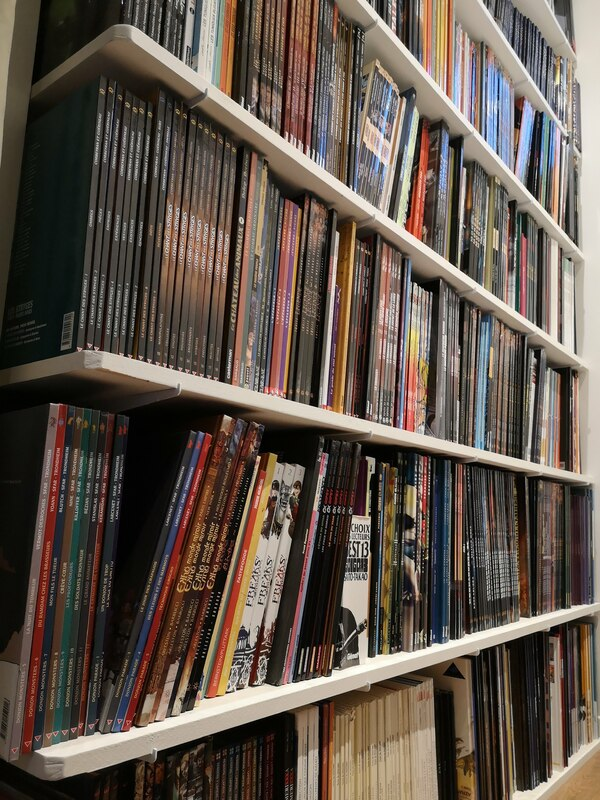
\includegraphics[width=3cm]{ressources/biblio.jpg}
\captionof{figure}{Bibliothèque}
\label{biblio}
\end{figure}

\begin{center}
\shadowbox{\parbox{17cm}{\centering Quelle solution peut-on mettre en place pour gérer efficacement la collection de bandes dessinées?}}
\end{center}
\section{Première approche}
La première approche imaginée consiste en l'utilisation d'un tableur (figure \ref{tableur}) pour stocker les informations.
\begin{figure}[!h]
\centering
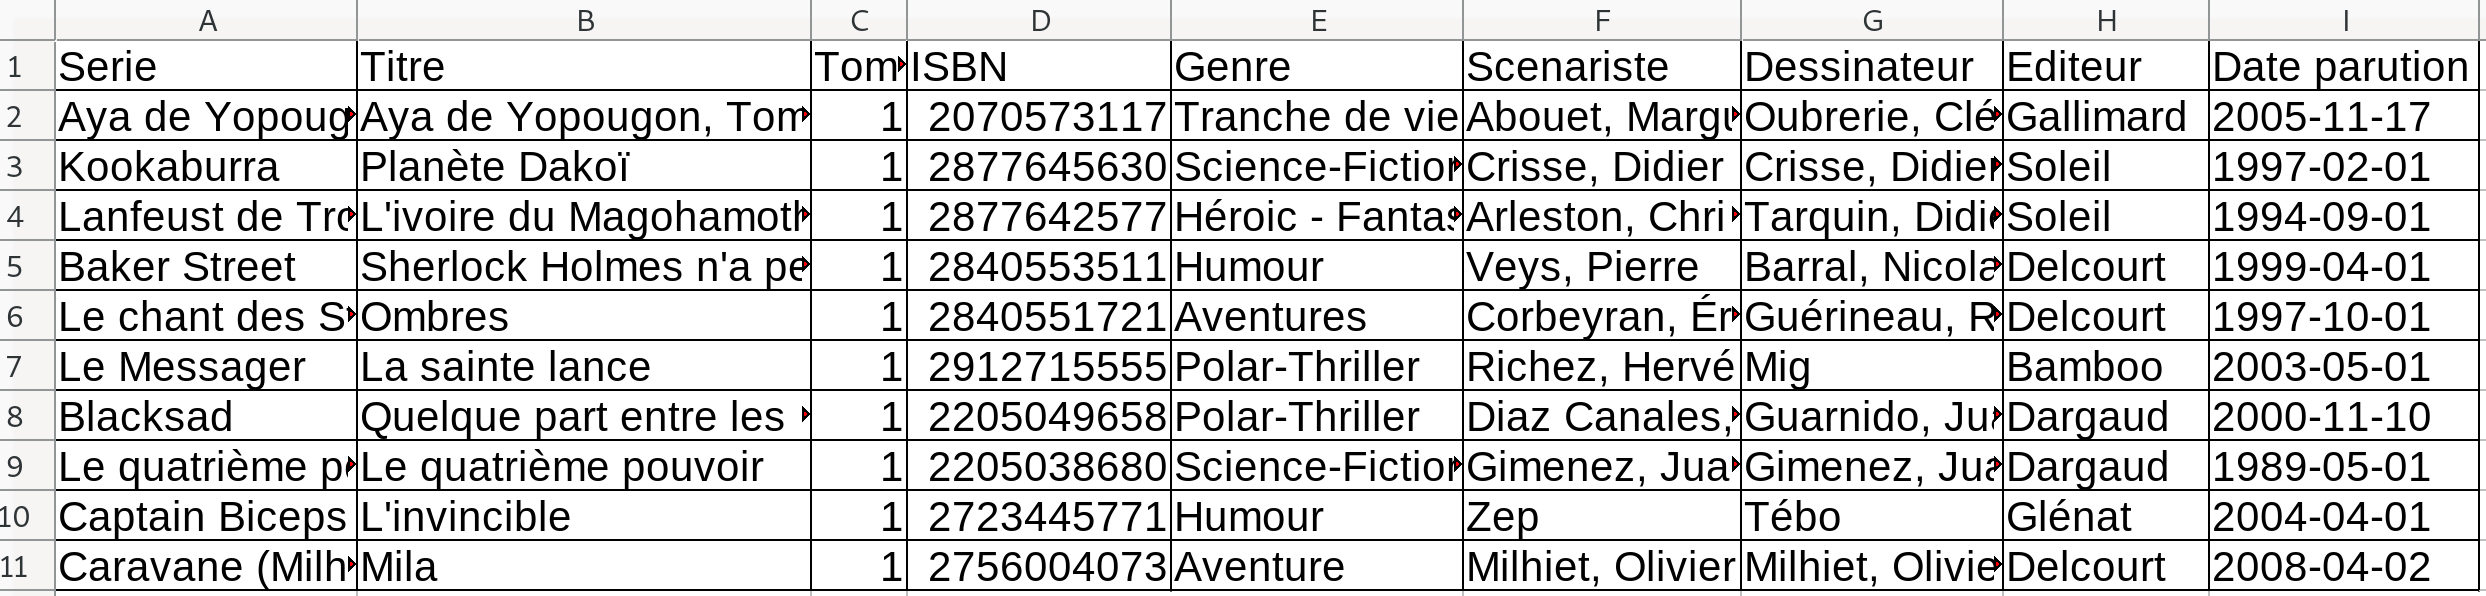
\includegraphics[width=15cm]{ressources/approche-1.png}
\captionof{figure}{Utilisation d'un tableur}
\label{tableur}
\end{figure}

Dans ce tableau, l'ajout d'une colonne \emph{emprunteur} permettrait de gérer les prêts.
\begin{activite}
Établir les limites de cette approche.
\end{activite}
\begin{commentprof}
\begin{itemize}
\item 2000 entrées = gérables par Python, mais si on veut étendre notre système à structure plus importante?
\item comment gérer modifications efficacement (ex: changement titre d'une série?)
\item Si on veut plus d'infos sur l'emprunteur (nom, date anniversaire, nb BD empruntées), les colonnes ajoutées sont-elles pertinentes dans ce tableau? Quand il rend un livre il faut vérifier/modifier beaucoup de lignes.
\item Que se passe-t-il si on change le titre d'une BD? L'emprunteur a-t-il vraiment pris ce livre?
\end{itemize}
\end{commentprof}
\section{Modèle de données}
\subsection{Modèle relationnel}
La première étape est de définir la manière dont les données vont être représentées. Le \emph{modèle relationnel} est un des plus populaires. Dans ce modèle théorique:
\begin{itemize}
\item Une \textbf{entité} est un objet représenté par un n-uplet de valeurs scalaires. Une bande dessinée est une \emph{entité}:
\begin{center}
(Captain Biceps, L'invincible, 1, 2723445771, Humour, Zep, Tébo, Glénat, 2004-04-01)
\end{center}
\item Une \textbf{relation} est l'ensemble des entités. On parle aussi de \emph{table}. La collection  de bandes dessinées est une \emph{relation}:
\begin{center}
(Captain Biceps, L'invincible, 1, 2723445771, Humour, Zep, Tébo, Glénat, 2004-04-01),\\
\small{(Caravane, Mila, 1, 2756004073, Aventure, Milhiet Olivier, Milhiet Olivier, Delcourt, 2008-04-02)},\\
(Kick-Ass, Le premier vrai super-héros, 1, 2809409994, Comics, Millar Mark, Romita Jr John, Panini Comics, 2010-03-17)

\end{center}
\item Une \emph{relation} possède des \textbf{attributs}. La relation des bandes dessinées possède les attributs:
\begin{center}
(serie, titre, tome, isbn, genre, scenariste, dessinateur, editeur, date\_parution)
\end{center}
\item Chacun de ces attributs est défini dans un domaine.
\begin{center}
\begin{tabular}{|cc|}
\hline 
\multicolumn{2}{|c|}{bandes\_dessinees} \\ 
\hline 
serie & String \\ 
titre & String \\ 
tome & Integer \\ 
isbn & String \\ 
genre & String \\ 
scenariste & String \\ 
dessinateur & String \\ 
editeur & String \\ 
date\_parution & Date \\ 
\hline 
\end{tabular} 
\captionof{code}{\textbf{Schéma} de la relation bandes\_dessinees}
\end{center}
\end{itemize}
\begin{commentprof}
scalaire = atomique\\
ISBN est un String car:
\begin{itemize}
\item certains ISBN-10 ont des lettres (cf back world)
\item ISBN-13 de la forme 978-2723452144 (avec un tiret)
\end{itemize}
\end{commentprof}
\begin{activite}
Sur le même modèle définir la relation des emprunteurs.
\end{activite}
\begin{commentprof}
la relation \emph{emprunteurs}: on pourrait encore mieux faire (le décompte des emprunts dans une autre table)
\subsection*{Contexte historique}

\end{commentprof}

\end{Form}
\end{document}